\chapter{AI Component}
\label{chap:ai-component}

\section{Business Context & AI Integration}
\label{section:business-context-and-AI-integration}
\textbf{Objective:}

\begin{figure}[h]
    \centering
    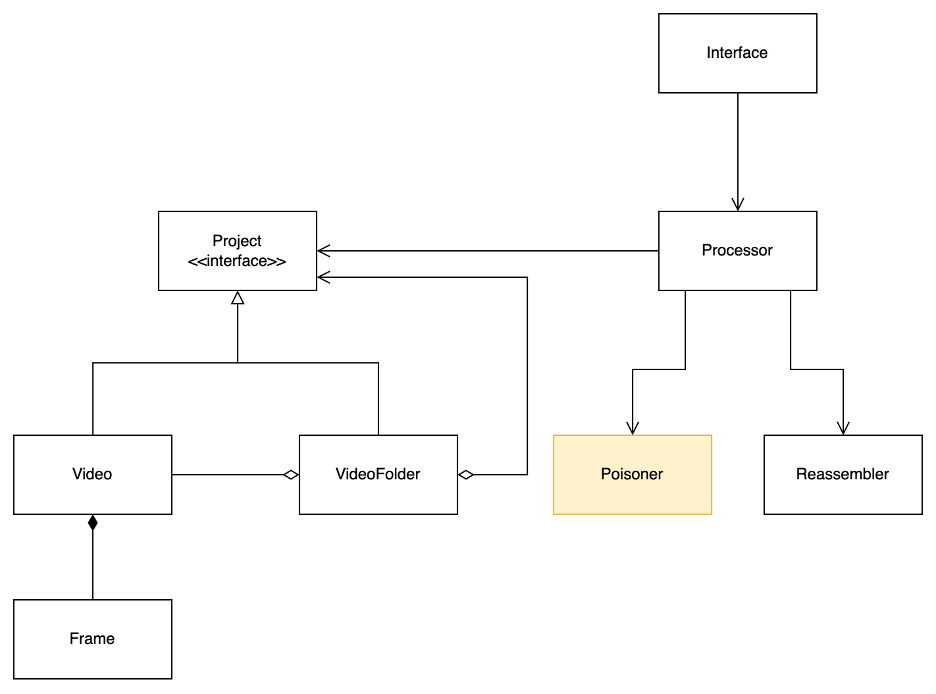
\includegraphics[width=0.8\textwidth]{chapter_5/Domain_Diagram.png}
    \caption{System's Domain Diagram}
\end{figure}

This is the system's domain diagram. The Poisoner component represents the part where AI will be used to generate adversarial perturbations to be injected into the frames of input videos.

AI is suitable for this task because the "poison" needs to understand how the AI sees images, in particular, the feature weights that influence its decision-making process. 

By injecting adversarial perturbations that manipulate the AI’s perception, we aim to cause the AI to misinterpret the images, distorting their true meaning as much as possible, while remaining perceptually similar to the human eye, by using the adversarial attack algorithm.

With this method, we can ensure that the poisoning method remains robust against AI training, continuing to degrade its performance even as AI learns from more images.

\section{Goal Hierarchy}
\label{section:goal-hierarchy}

\subsubsection{Organization Goals}
\begin{enumerate}
    \item 
    \textbf{Goal:}
    Discouraging anyone from using creator's intellectual property in non-consensual AI training. \\
    \textbf{Measured by:} 
    Reduction in cases of unauthorized AI usage reported by creators. \\
    \textbf{Data collection:}
    Amount of successfully removed artist's name and work from AI training datasets due to adversarial attacks that break the AI's ability to replicate the artist style. \\
    \textbf{Operationalization:} 
    Evaluate AI ability to replicate the artist style before and after poisoning using similarity metrics and model accuracy. Track the number of models where the artist data becomes unusable or is successfully excluded.
\end{enumerate}

\subsubsection{System Goals}
\begin{enumerate}
    \item 
    \textbf{Goal:}
    Process various video formats and inject adversarial perturbations with minimal perceptual change. \\
    \textbf{Measured by:} 
    Percentage of processed videos meeting quality and poisoning effectiveness standards. \\
    \textbf{Data collection:}
    System logs of predictions and User feedback. \\
    \textbf{Operationalization:} 
    Evaluate processed videos using perceptual similarity metrics and poisoning effectiveness.
\end{enumerate}

\subsubsection{User Goals}
\begin{enumerate}
    \item 
    \textbf{Goal:}
    Provide users with confidence that their content remains visually unchanged while being protected. \\
    \textbf{Measured by:} 
    User satisfaction ratings and survey feedback. \\
    \textbf{Data collection:}
    Post-processing surveys, user feedback forms, and visual comparison ratings (original vs. poisoned). \\
    \textbf{Operationalization:} 
    Collect and analyze survey results periodically to assess perceived visual quality. Adjust perturbation strength or method based on recurring feedback trends.
\end{enumerate}

\subsubsection{AI Model Goals}
\begin{enumerate}
    \item 
    \textbf{Goal:}
    Generate adaptive adversarial perturbations tailored to each video's unique features (light, color, texture, etc.). \\
    \textbf{Measured by:} 
    Percentage of processed videos meeting quality and poisoning effectiveness standards. \\
    \textbf{Data collection:}
    AI model history and User feedback. \\
    \textbf{Operationalization:} 
    Test perturbations across multiple AI models and log evasion success rates. Analyze perturbation patterns against video feature distributions (e.g., lighting, color).
\end{enumerate}


\section{Task Requirements Analysis Using AI Canvas}
\label{section:task-requirements-analysis-using-AI-canvas}
\subsection{AI Task Requirements}

\subsubsection*{Requirements (REQ)}
\begin{itemize}
    \item REQ-1: The AI must generate adversarial examples from input images using the FGSM technique.
    \item REQ-2: The AI should ensure poisoned images cause significant misclassification in target neural network models.
    \item REQ-3: The poisoning should preserve visual integrity such that it remains perceptually similar to the original.
    \item REQ-4: The AI must support batch processing for datasets.
\end{itemize}

\subsubsection*{Specifications (SPEC)}
\begin{itemize}
    \item SPEC-1: The AI uses the Adversarial Robustness Toolbox (ART) to implement FGSM attacks.
    \item SPEC-2: The perturbation strength $\epsilon$ should be configurable by the user.
    \item SPEC-3: Poisoning will be applied directly to image tensors prior to model training.
\end{itemize}

\subsubsection*{Environment (ENV)}
\begin{itemize}
    \item ENV-1: The system runs in a Python environment (e.g., Jupyter or Colab) with TensorFlow or PyTorch backends.
    \item ENV-2: Input data consists of image files (.jpg, .png)
    \item ENV-3: Requires GPU acceleration for efficient batch poisoning.
    \item ENV-4: May be extended later for use in video frame sequences.
\end{itemize}

\subsection{AI Canvas Development}

\begin{table}[h]
\centering
\begin{tabular}{|p{4cm}|p{10cm}|}
\hline
\textbf{Canvas Element} & \textbf{Description} \\
\hline
\textbf{Input Data} & Raw image files. Input will be uploaded manually. \\
\hline
\textbf{Expected Output} & Poisoned images with imperceptible perturbations that cause target models miss understand. \\
\hline
\textbf{Tools/Frameworks} & Python, ART, TensorFlow or PyTorch, NumPy, Google Colab or local machine with GPU. \\
\hline
\textbf{Success Criteria} & 
\begin{itemize}
    \item Target models miss understand the feature.
    \item No noticeable visual difference in the poisoned training images (PSNR > 30dB).
\end{itemize} \\
\hline
\end{tabular}
\end{table}

\section{User Experience Design with AI}
\label{section:user-experience-design-with-AI}


\subsection{Interaction Style}
\textbf{Interaction Style: Annotate}

\begin{itemize}
    \item The AI modifies and tags poisoned images with visual indicators (e.g., warning labels).
    \item Users are informed when images are altered for adversarial purposes.
    \item This method provides transparency and keeps the user in control.
\end{itemize}

\subsection{User Feedback Mechanism}
Users are encouraged to provide feedback to help improve the AI poisoning system. The application offers a dedicated \textbf{Feedback} dropdown menu with the following options:
\begin{itemize}
    \item \textbf{Comments and Suggestions} – Share thoughts or ideas for improving the poisoning algorithm.
    \item \textbf{Bug Reports} – Report technical issues or incorrect behavior in the poisoning process.
    \item \textbf{Email Us} – Directly contact the development team for in-depth support.
\end{itemize}

\subsection{AI Contribution to System Intelligence}

This system integrates AI to perform intelligent poisoning of image data. 
This AI component significantly enhances the system’s capabilities beyond what 
is possible with non-AI approaches.

\subsubsection{Without AI Integration}
\begin{itemize}
    \item Manual image editing to distort data.
    \item Watermarking or fixed filters that are easily bypassed by neural networks.
\end{itemize}

\subsubsection{With AI Integration}
\begin{itemize}
    \item Automated poisoning of images based on gradient information.
    \item Adaptability to different neural network architectures.
    \item Preservation of visual quality for human viewers while deceiving models.
    \item Scalable batch processing of datasets with consistent adversarial effectiveness.
\end{itemize}
